\documentclass[border=0.8ex,svgnames,tikz]{standalone}
\usepackage{amsmath,mathtools}
\usepackage{fontspec}
\setmainfont{Source Serif 4}
\setsansfont{Source Sans 3}
\setmonofont{Source Code Pro}

\usetikzlibrary{positioning,calc}

\begin{document}
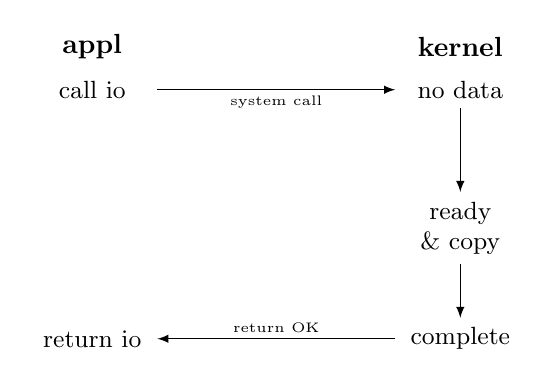
\begin{tikzpicture}
  \coordinate(appl) at (0,0);
  \coordinate(kernel) at ($(appl)+(13.3em,0)$);
  \begin{scope}[
    every node/.style={
      align=center,
      anchor=center,
      font=\small,
      text width=4em,
    },
    ]
    \path[draw=none] node(noready){no data}
    ++(0,-5em) node(ready){ready \& copy}
    ++(0,-4em) node(complete){complete};
    \node (call)   at ($(noready)-(kernel)-(appl)$)   {call io};
    \node (return) at ($(call)+(complete)-(noready)$) {return io};
  \end{scope}
  \begin{scope}[
    every node/.style={font=\tiny,inner sep=0.45ex},
    every path/.style={draw,>=latex},
    ]
    \path[->]
    (call) edge node[below]{system call} (noready)
    (noready) edge (ready)
    (ready) edge (complete)
    (complete) edge node[above]{return OK} (return);
  \end{scope}
  \node[above=1ex of call,inner sep=0ex](appl-label){\bfseries appl};
  \node at ($(appl-label)+(kernel)-(appl)$) {\bfseries kernel};
\end{tikzpicture}
\end{document}
